\begin{figure*}[h]                                                           
 
\includegraphics[width=\linewidth]{./media/images/murder}%
%  \scriptsize{\textsc{\\This is} the article main image caption.}
  \label{fig:editorial}%                                                 
\end{figure*}                                                                
\begin{quotation} 
\noindent\color{Sepia}{{\textit{\textbf{“To catch a killer, one must think like a killer”}}}}\\[.5mm]
%remove following line space if you're tight on vertical room and need to fit on
%single page

\hfill\color{Sepia}{\small{\textendash \textsc{Belinda Bauer, The Beautiful Dead}}}
\end{quotation} 
\newpage
Felicity Banks recently published her new work, \emph{Magic in the Mail}.
\emph{Magic} is a ``whodunnit'' where you receive pretty cool stuff, I must say,
through the mail. We exchanged emails for this interview.
\medskip

\emph{Felicity Banks, you've written novels as well as writing for Tin Man Games and others. What made you invent a system as unique as Murder in the Mail and Magic in the Mail?}
\medskip

I've been cheerfully telling other novelists that they can get quite a decent advance for writing IF, and my print publisher (Odyssey Books) asked me to write something interactive that could be part of the new imprint, Publisher Obscura, which is all about picture books for adults. One thing led to another and once I had a solid idea (or three) I was unable to let it go. 

\medskip
\emph{Can you tell us how these stories work?}

\medskip
At present there are two stories, and one in development. I originally chose crime because whodunnit books already have a puzzle element for the canny reader. So in the story Murder in the Mail: A Bloody Birthday, a girl named Naomi is killed at her own birthday party. It's clear that one of her friends is the killer, and they're all artists... so "you" have asked them to send you both their suspicions of one another and their artworks done around the time of the murder.

I hired six artists and six writers, so each character in the story has their own voice and their own artistic style. Every picture contains clues about the identity of the killer (and of course the secrets of the other characters). So it's a sampler of authors and artists as well as a story and a puzzle (although I am too merciful to leave readers unsure of the answers, so it resolves as neatly as a regular book).

In the subscription version of the story (only available in Australia now, sorry) the reader receives a parcel each week containing a letter, a postcard, at least one physical object, and a piece of art. The physical objects are also clues about the killer, and are carefully chosen to involve all the reader's senses.

The story will be converted into a 'normal' book in 2019, so it's only available for a limited time.

\medskip
\emph{You mentioned Magic in the Mail? What's that?}

\medskip
There is a full-length Magic in the Mail story in development that still has a minor puzzle element as well as a wider range of art (a hand-printed silk bookmark and things like that). . . but in the meantime I wrote a Magic in the Mail mini-story called Emmeline's Empire that is a steampunk fantasy love story between two women. It includes jewellery, a castle for the reader to build, and a sing by the Littmus Steampunk Band.

\medskip
\emph{Shut up and take my money!}

\medskip
Okay. The store is at MurderintheMail.net/store.
\bigskip
\marginnote{\href{http://ifdb.tads.org/search?searchbar=Felicity+Banks&searchGo.x=0&searchGo.y=0}{Felicity Banks' Interactive Fiction Database page}}[3em]
\begin{wrapfigure}{l}{0.45\textwidth}
  \vspace{-2em}
  \begin{center}
  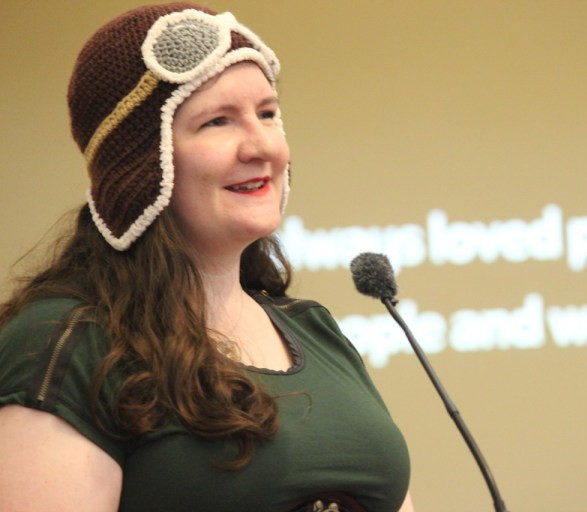
\includegraphics[width=\linewidth]{./media/images/felicity}%
%  \scriptsize{\textsc{\\This is} the article main image caption.}
  \label{fig:brian}%
  \end{center}
\end{wrapfigure}                                                                
\noindent\emph{Felicity Banks has several novels published with Odyssey Books (a small press in
Australia) and is a minion of Tin Man Games (being heavily involved with their
\emph{choices that matter} serial story app on iOS and Google Play) as well as
various other things (all listed on her ifdb page). Felicity's ChoiceScript tale, \emph{Scarlet Sails}, placed 7th in the 2015 IF Comp.}